\documentclass[aspectratio=169]{beamer}

\usetheme{Madrid}
\usepackage{amsmath, amssymb}
\usepackage{booktabs}
\usepackage{graphicx}
\graphicspath{{../}{./}}

% \section[short]{full}: the short form appears in the outline and in the
% Madrid headline/footline; the full form titles the section itself.

\title[Crossover Disambiguation]{Crossover Disambiguation in Kuramoto Sequential Memory}
\subtitle{Learning rules for branch-ambiguous retrieval in oscillator dense associative memory}
\author{}
\institute{}
\date{}

\begin{document}

\begin{frame}
  \titlepage
\end{frame}

\begin{frame}{Outline}
  \tableofcontents
\end{frame}


% =====================================================================
\section[Introduction]{Introduction and Motivation}
% =====================================================================

\begin{frame}{Sequential retrieval in associative memory}
  \begin{itemize}
    \item
    \item
  \end{itemize}
\end{frame}

\begin{frame}{The crossover problem}
  \framesubtitle{Overlapping sequences share a state; the transition rule is symmetric in the branches}
  \begin{itemize}
    \item
  \end{itemize}
\end{frame}

\begin{frame}{Objectives}
  \begin{itemize}
    \item
  \end{itemize}
\end{frame}

\begin{frame}{Model overview}
  \framesubtitle{Kuramoto dense associative memory and the energetic formulation}
  \begin{itemize}
    \item
  \end{itemize}
\end{frame}


% =====================================================================
\section{Literature Review}
% =====================================================================

\begin{frame}{Foundations: associative and dense memory}
  \begin{itemize}
    \item Krotov \& Hopfield --- higher-order interactions, dense capacity
    \item
  \end{itemize}
\end{frame}

\begin{frame}{Sequential memory: asymmetric couplings and transition matrices}
  \begin{itemize}
    \item
  \end{itemize}
\end{frame}

\begin{frame}{Open problem: crossover disambiguation}
  \begin{itemize}
    \item
  \end{itemize}
\end{frame}


% =====================================================================
\section[Model]{Model and Learning Rules}
% =====================================================================

\begin{frame}{Motivation for Kuramoto dynamics}
  \framesubtitle{Smooth retrieval trajectories and physically realizable coupling}
  \begin{itemize}
    \item
    \item
  \end{itemize}
\end{frame}

\begin{frame}{Baseline learning rule}
  \[
  \]
\end{frame}

\begin{frame}{Sequence retrieval algorithm}
  \begin{itemize}
    \item
  \end{itemize}
\end{frame}

\begin{frame}{Single-sequence retrieval under the baseline rule}
  \centering
  % 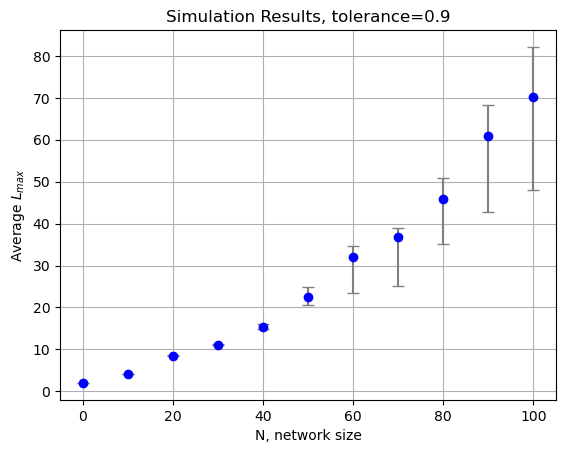
\includegraphics[width=0.7\textwidth]{outputs/output.png}
\end{frame}

\begin{frame}{Failure of the baseline rule at a crossover}
  \centering
  % 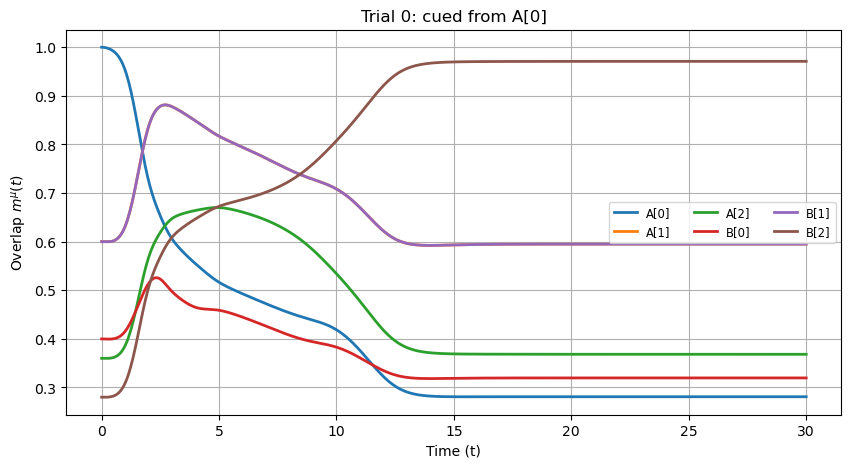
\includegraphics[width=0.7\textwidth]{outputs/crossover_vanilla.png}
\end{frame}

\begin{frame}{Symmetry of the energy landscape}
  \begin{itemize}
    \item
  \end{itemize}
\end{frame}

\begin{frame}{Heterogeneous lag-context learning rules}
  \begin{itemize}
    \item
  \end{itemize}
\end{frame}


% =====================================================================
\section[Results]{Numerical Experiments and Results}
% =====================================================================

\begin{frame}{Benchmark design}
  \framesubtitle{Crossover geometries and scoring criteria}
  \begin{itemize}
    \item
  \end{itemize}
\end{frame}

\begin{frame}{Catalogue of learning rules}
  \centering
  \begin{tabular}{ll}
    \toprule
    Rule & Gate \\
    \midrule
     & \\
     & \\
    \bottomrule
  \end{tabular}
\end{frame}

\begin{frame}{Experimental conditions and parameters}
  \begin{itemize}
    \item
  \end{itemize}
\end{frame}

\begin{frame}{Crossover resolution across the rule catalogue}
  \begin{itemize}
    \item
  \end{itemize}
\end{frame}

\begin{frame}{Superposition of learning rules}
  \begin{itemize}
    \item
  \end{itemize}
\end{frame}

\begin{frame}{Robustness: corruption rate and network size}
  \centering
  % 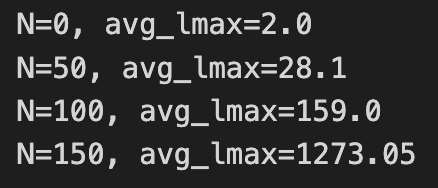
\includegraphics[width=0.5\textwidth]{outputs/large_N.png}
\end{frame}

\begin{frame}{Discussion: rule performance and limitations}
  \begin{itemize}
    \item
  \end{itemize}
\end{frame}


% =====================================================================
\section[Analysis]{Theoretical Analysis}
% =====================================================================

\begin{frame}{Tensor formulation: symmetric and asymmetric components}
  \begin{itemize}
    \item
  \end{itemize}
\end{frame}

\begin{frame}{Scalability and capacity}
  \begin{itemize}
    \item
  \end{itemize}
\end{frame}


% =====================================================================
\section[Conclusions]{Conclusions and Outlook}
% =====================================================================

\begin{frame}{Conclusions}
  \begin{itemize}
    \item
  \end{itemize}
\end{frame}

\begin{frame}{Applications}
  \framesubtitle{Oscillator-based hardware and neurobiological sequence memory}
  \begin{itemize}
    \item
    \item
  \end{itemize}
\end{frame}

\begin{frame}{Outlook and open questions}
  \begin{itemize}
    \item
  \end{itemize}
\end{frame}

\end{document}
